\documentclass[]{beamer}
\usepackage[framemethod=tikz]{mdframed}
\usepackage{pgfplots}
\usepackage{tikz}
\usepackage{url}
\usepackage{xcolor}
\usepackage{xmpmulti}
\usetikzlibrary{shapes,arrows}
\hypersetup{pdfstartview={Fit}} % Fit the presentation to the window when first displayed
\usetheme{Frankfurt}
\pgfplotsset{compat=1.14}
\beamertemplatenavigationsymbolsempty{} % Remove Beamer navigation symbols
\nonstopmode{} % Keep making the file through errors
\usepackage[sfdefault]{sourcesanspro}
\usepackage[T1]{fontenc}

% http://danielfalster.com/blog/2013/06/18/a-nice-title-page-for-beamer-presentations/
\newmdenv[tikzsetting={draw=black,fill=white,fill opacity=0.7, line width=1pt},backgroundcolor=none,leftmargin=0,rightmargin=0,innertopmargin=5pt,skipbelow=\baselineskip,skipabove=\baselineskip]{TitleBox}

\title{Open Circuit: \\Printed Circuit Boards and Free Software}
\author[Swartz]{Tom~Swartz}
\institute{Central PA Open Source Conference 2019}
\date{September 21 2019}
\subject{Computer Science}
\begin{document}

% Title Page
{\usebackgroundtemplate{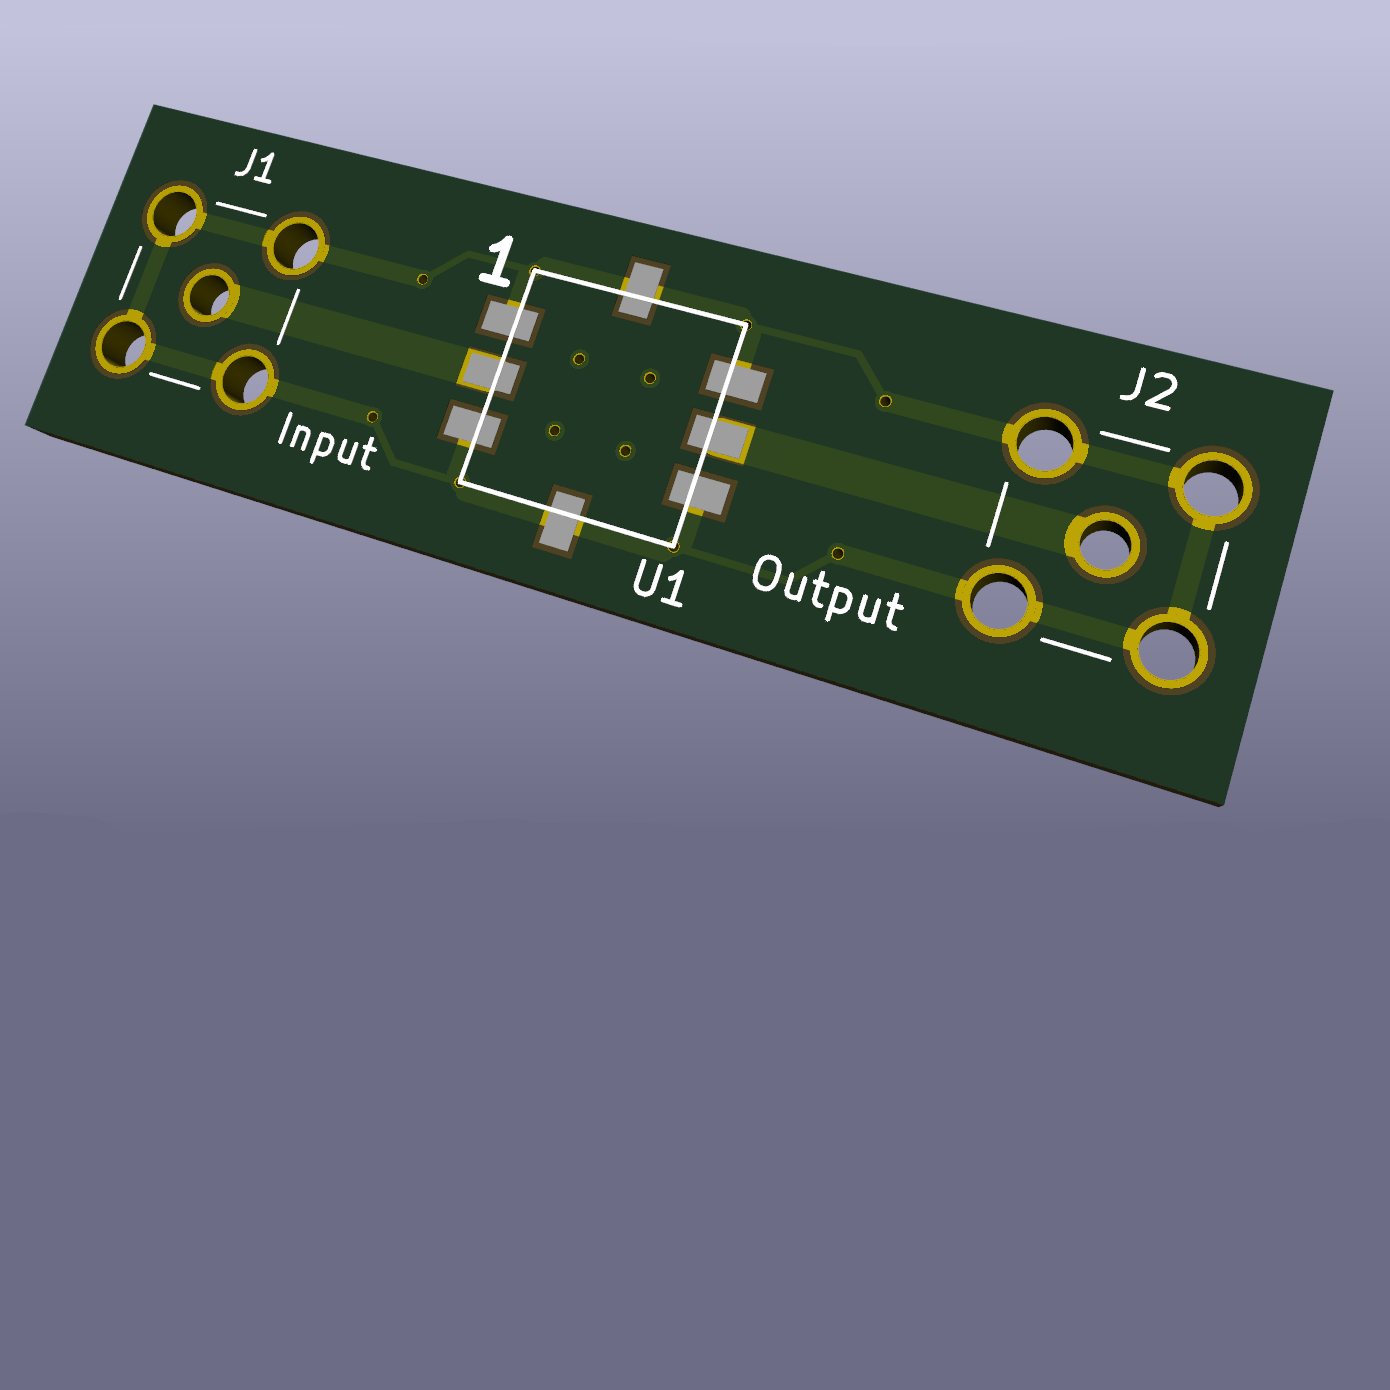
\includegraphics[height=1.00\paperwidth,keepaspectratio]{images/kicad3d.png}}
\begin{frame}[plain]
    \vspace{17em}
    \begin{TitleBox}
        \begin{center}
            {\color{red}\Large\inserttitle\color{black}}\\
        \end{center}
        \insertauthor{}\hfill\insertinstitute{}\\
        {\footnotesize
        \href{http://twitter.com/tswartz07}{@tswartz07}
        \hfill
        \href{mailto: tom@tswartz.net}{tom@tswartz.net}
        }
    \end{TitleBox}
\end{frame}}

\begin{frame}[plain]
    \frametitle{Who is this guy?}
    \framesubtitle{And what is he doing here?}
    \begin{columns}[T]
        \begin{column}[T]{5cm}
           {\huge Tom Swartz}
            \begin{itemize}%[<+->]
                \item{Hobbist hardware hacker}
                \item{Make PCBs for various personal projects}
            \end{itemize}
        \end{column}
        \begin{column}[T]{5cm}
            
\includegraphics[height=6cm]{images/me.jpg}
        \end{column}
    \end{columns}
\end{frame}

% What's ahead?
\begin{frame}[plain]
    \frametitle{Agenda}
    \tableofcontents
\end{frame}

\section[Background]{Background}
\subsection[But Why?]{Why make your own circuit boards?}
\begin{frame}
    \frametitle{\insertsection{} Outline}
    \begin{itemize}
        \item For finishing projects
        \item Project evolution- Perfboard $\rightarrow{}$ PCB
        \item Intro to KiCAD
    \end{itemize}
\end{frame}
\subsection[KiCAD]{Introduction to KiCAD}
\begin{frame}
    \frametitle{\insertsection{} Outline}
    \begin{itemize}
        \item Intro to KiCAD
        \item Overview of EDA programs
    \end{itemize}
\end{frame}

\section[Design]{Designing a Schematic}
\begin{frame}
    \frametitle{\insertsection{} Outline}
    \begin{itemize}
        \item Start small
        \item Test prototype
        \item Get datasheets
        \item KiCAD drawings
    \end{itemize}
\end{frame}

\section[Layout]{Creating a PCB Layout}
\begin{frame}
    \frametitle{\insertsection{} Outline}
    \begin{itemize}
        \item Lay out the rats nest
        \item Find the matching parts
        \item Place parts
        \item Zones- ground planes, power rails, etc
    \end{itemize}
\end{frame}

\section[Fabrication]{Preparing for Factory Fabrication}
\begin{frame}
    \frametitle{\insertsection{} Outline}
    \begin{itemize}
        \item Each PCB Fab house is different, but general rules apply
        \item Gerber Files
        \item General limits and tolerances
        \item Exporting files, loading them to Fab house
    \end{itemize}
\end{frame}

\section[Post-Production]{Post-Production}
\begin{frame}
    \frametitle{\insertsection{} Outline}
    \begin{itemize}
        \item General info on how quick process is
        \item Receiving the boards
        \item Testing boards for defects, issues from design
        \item Populating the boards
        \item Profit
    \end{itemize}
\end{frame}

\end{document}

% vim: set ts=4 sw=4:
